\documentclass{unswmaths}
\usepackage{unswshortcuts}
\usepackage{hyperref}
\begin{document}
\author{Adam J. Gray}
\title{Assignment 2}
\subject{Ergodic Theory}
\studentno{3329798}

\unswtitle

\section{}
\subsection{}
\begin{align*}
    T(\theta, \nu) = (\theta + \nu \mod 2\pi, \alpha\nu + \gamma \cos(\theta + \nu))
\end{align*}
\subsection{}
In any neighbourhood not around $ 2n\pi $ for $ n \in \mathbb{Z} $ we have that
\begin{align*}
    J[T](\theta, \nu) = \left( 
    \begin{array}{cc}
        1   & 1 \\
        -\gamma \sin(\theta + \nu) & \alpha - \gamma\sin(\theta + \nu)
    \end{array}
    \right)
\end{align*}
and so
\begin{align*}
|J[T](\theta, \nu)| &= \alpha - \gamma\sin(\theta + \nu) + \gamma\sin(\theta + \nu) \\
    &= \alpha.
\end{align*}
So $ |J[T](\theta, \nu)| = 0 $ iff $ \alpha = 0 $. So since we have chosen $ \alpha > 0 $ this map is invertible everywhere except around at $ 2n\pi $ by the inverse function theorem.
\subsection{}

See code in \emph{Question\_3.m} available at \url{https://github.com/adamjoshuagray/Honours_Ergodic_Theory/tree/master/Assignment_2/Project_1_Code}.
\begin{figure}[h]
    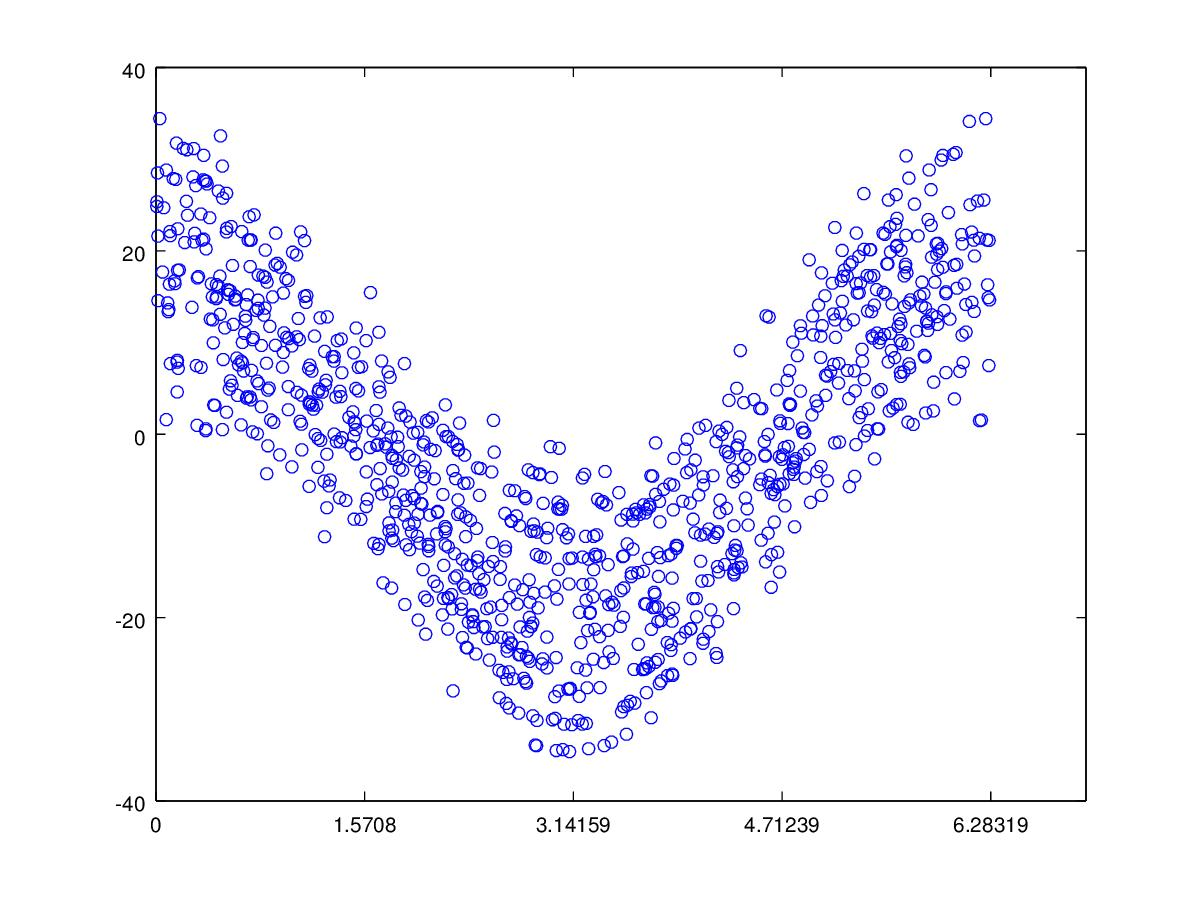
\includegraphics[scale=0.5]{Question_3}
    \caption{Phase plot of velocity vs table phase with $ \theta_0 = 0.5, \nu_0 = 0.5 $}
\end{figure}
\subsection{}
The maximum post-bounce velocities occur near $ \theta = 0 $ ($\theta = 2\pi$). This makes sense because the piston is travelling in the opposite direction to the ball. This is happening fastest at $ \theta = 0 $ and so this results in the largest bounces. The minimum is found at $ \theta = \pi $. This also makes sense because this is when the piston is travelling in the same direction as the ball. This is happening fastest at $ \theta = \pi $ and this results in the largest slowdown in the bounce.

\subsection{}
This does not preserve Lebesgue measure. To see why consider $ \Omega = [\frac{\pi}{2}, \pi] \times [1,2] $ and note that $ \mu(\Omega) = \frac{\pi}{2} $. It is clear to see, however, that $$ T^{-1}T(\Omega) \supseteq [\frac{\pi}{2},\pi] \times [1,2] \cup [\pi, \frac{3\pi}{2}] \times [1,2]$$ and thus $$ \mu(T^{-1}T(\Omega)) \geq 2 \mu(\Omega) $$ and hence this map does not preserve Lebesgue measure.
Is this a contradiction of ergodicity and mixing? No. While an ergodic map must be measure preserving, there is no requirement that it preserves the Lebesgue measure specifically. 
\subsection{}

See code in \emph{Question\_6.m} available at \url{https://github.com/adamjoshuagray/Honours_Ergodic_Theory/tree/master/Assignment_2/Project_1_Code}.
\label{qn_6_ergodic}
\begin{figure}[h]
    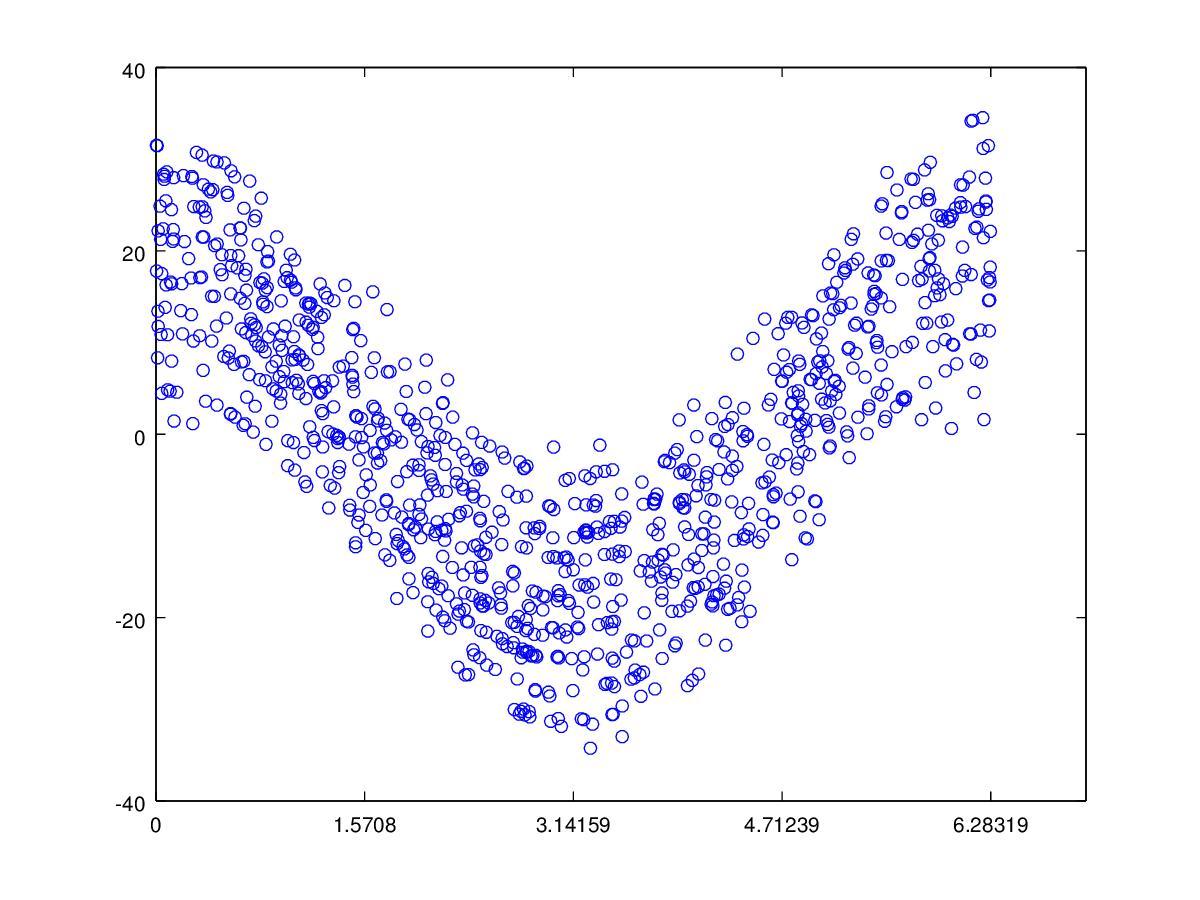
\includegraphics[scale=0.5]{Question_6_Ergodic}
    \caption{A bundle of 1000 points starting near $ \theta_0 = 0.5,  \nu_0 = 0.5 $ were iterated through $  T $ 10000 times}
\end{figure}

What figure 2 shows is that a small ball of points \emph{spreads out} in the phase space. Note that this ensemble of points roughly matches the orbit of one point. This would lead us to suspect that this process is Ergodic. 

\clearpage
\begin{figure}[h]
    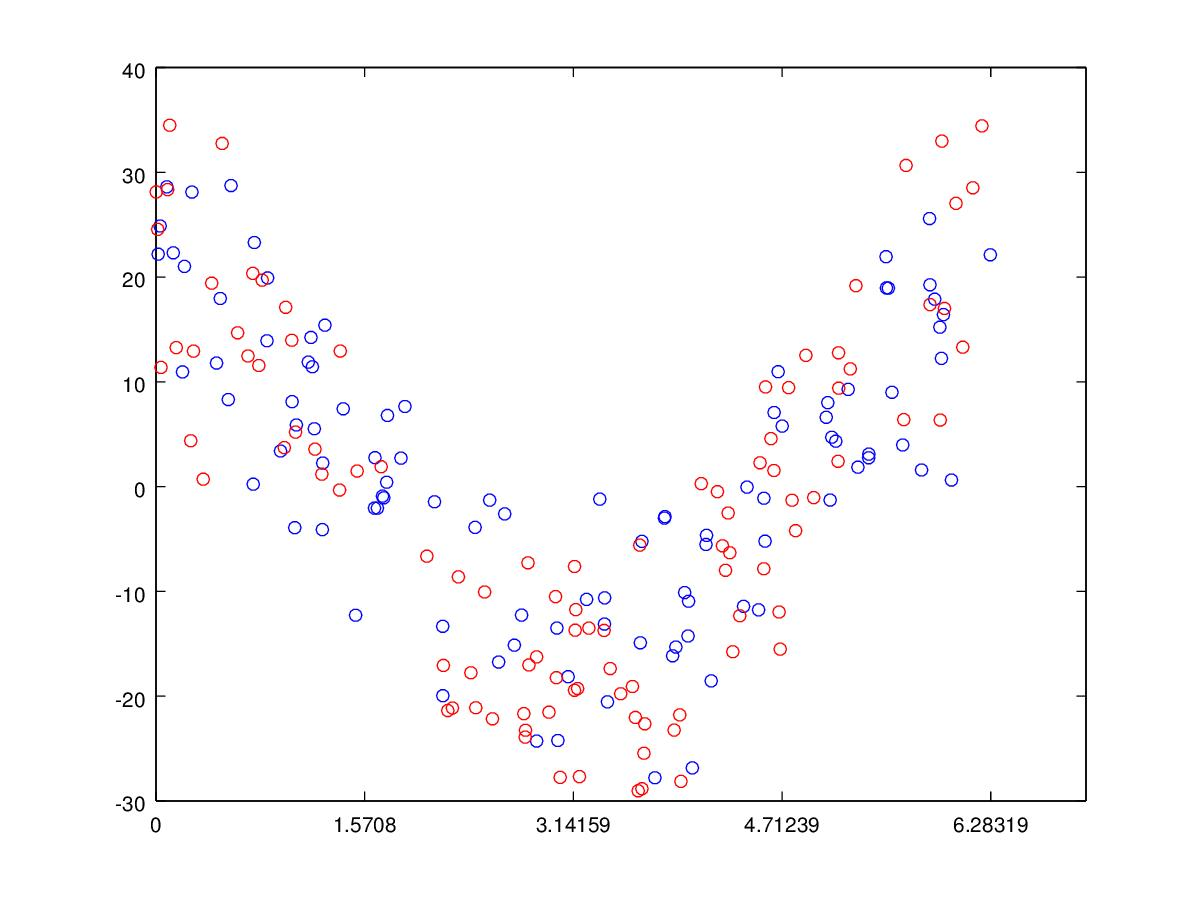
\includegraphics[scale=0.5]{Question_6_Mixing}
    \label{qn_6_mixing}
    \caption{Two bundles of 200 points after iterating through  $ T $ 10000 times. Blue started near $ \theta_0 = 0.5, \nu_0 = 0.5 $ while red started near $ \theta_0 = 1, \nu_0 = 1 $ }
\end{figure}


Figure 3 suggests that the long term behaviour of the  points is independent of their starting point. That is two sets of balls mix together. Although only testing with two bundles of balls is hardly rigorous, even empirically, this would suggest that this process is mixing.
\subsection{}

See code in \emph{Question\_7.m} available at \url{https://github.com/adamjoshuagray/Honours_Ergodic_Theory/tree/master/Assignment_2/Project_1_Code}.
Since we suspect that this process is Ergodic (and mixing) this question can be answered by watching the long term behaviour of 1 point. We do this for a point starting at $ \theta_0 = 0.5, \nu_0 = 0.5 $ and see that $ 49.95 \% $ of the first 10000 bounces occur when $ \theta < \pi / 2 $ or $ \theta > 3\pi / 2 $, that is when the piston is moving up. We conclude that there is equal chance of the ball hitting on a down stroke compared to an up-stroke.

\subsection{}

See code in \emph{Question\_8.m} available at \url{https://github.com/adamjoshuagray/Honours_Ergodic_Theory/tree/master/Assignment_2/Project_1_Code}.
Again since we suspect that this process is Ergodic we just study the evolution of one point.
We see that with $ \theta_0 = 0.5, \nu_0 = 0.5 $ the maximum $ \nu $ achieved is $ 34.821 $ and the 945 bounces are within $ 1\%$ of this velocity over $ 10^6 $ iterations. This suggests that ball is within $ 1\%$ of its maximum post bounce speed about $ 0.945\% $ of the time. 

The above paragraph is actually wrong. Let me explain. If we consider the distribution of $ \nu $ as shown in figure 4 we can see that by taking different orbit lengths we essentially get different values for the percentage of time that $ \nu $ is within $ 1\% $ of its observed maximum. This is because with an orbit length of say $ 10^4 $ we would get the first black line as the observed maximum whereas with $ 10^5 $ iterations we get the second black line as the observed maximum. We can easily see that the $ -1\% $ brackets of these two lines correspond to different parts of the distribution and therefore correspond to different observed percentages.
Precisely this problem occurs in the next two questions as well..


\begin{figure}[h]
    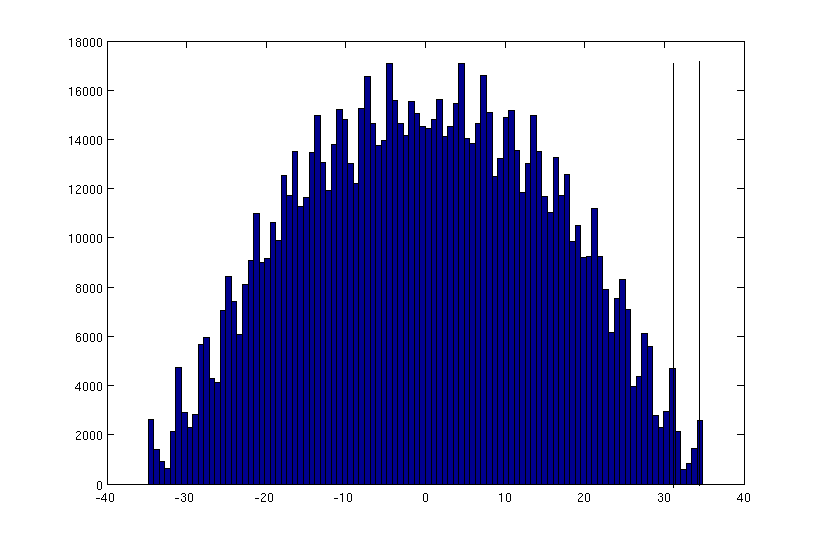
\includegraphics[scale=0.5]{nu_Histogram}
    \label{nu_Histogram}
    \caption{A histogram of $ \nu $ taken from $ 10^6 $ iterations of $ T $ starting at $ \theta_0 = 0.5 $ and $ \nu_0 = 0.5 $ }
\end{figure}

\subsection{}
See code in \emph{Question\_9.m} and \emph{Question\_9\_Empirical\_Measure.m} available at \url{https://github.com/adamjoshuagray/Honours_Ergodic_Theory/tree/master/Assignment_2/Project_1_Code}.


We use two numerical methods for calculating the expected return time and one numerical method. The first method is by saying $ \mathbb{E}[r] = \frac{N}{N_h + 1}$ where $ r $ is the return time, $ N $ is the number of iterations of the $ T $ map in the orbit and $ N_h $ is the number of times it falls within the region of interest. This uses the fact that we suspect $ T $ is ergodic to say that $ n$-th return times should be the same as the $ 1$-st return time.
Using this method with $ \theta_0 = 0.5, \nu_0 = 0.5 $ and using $ 10^6 $ iterations we get that $ \mathbb{E}[ r] = 1258 $.

We can also do a similar thing for an ensemble of $ 1000 $ points but only measuring the $1$-st return time (instead of every return). Doing this we get $ \mathbb{E}[r] = 1140 $. Notice that these two numbers are actually quite different. Despite the fact that we use the same orbit lengths ($10^6$) we most likely encountering this difference due to the issue outlined in the previous question.

We would like to look at the original problem, that is finding the expected return time of points to the $ [11.88\pi, 12\pi] $ we need to make some approximations to get anywhere with the problem. Firsly we notice that the points essentially lie in a band bounded by $ 12\pi\sin(\theta) $ and $ 12\pi\sin(\theta) - 12\pi $. This band has area $ 24\pi $. Now assuming that the points are uniformally distributed in the band (they are not) we are simply interested in the proportion of area of this band which has $ \nu > 11.88\pi $. Then by Kac's theorem we invert this to calculate the expected return time.

The calculations are as follows
\begin{align*}
    \cos(\theta) = \frac{11.88}{12}
\end{align*}
and thus $ \theta = 0.1415 $. 
Then the area in the left hand upper region is
\begin{align*}
    \pi \left( 12\int_0^{0.1415} \cos(\theta) d\theta - 11.88 * 0.1415\right) &= \pi \left( 12\sin(0.1411) - 11.88 * 0.1415 \right) \\
    &= 0.006567\pi.
\end{align*}
The area in the right hand upper region would be the same, and thus the proportion of area is $ ( 0.01313 \pi) / 24\pi \approx 0.0005473 $ and thus by Kac's theorem we have that the expected return time is $ 1 / 0.0005473 = 1827 $. Numerical simulations show that it is much much worse than this. 
This is a good \emph{rough estimate} of how things could be, based on the assumption that all the point fall in a band and are uniformally distributed in the band. This is not the case because not all points do fall in the band and the distribution is not uniform as shown by the 2 dimensional histogram in figure 5. This shows that there is a clear banding on the distribution and so it is not uniform across the distribution. 

We should make clear that in searching for the points in the region $ \nu \in [11.88\pi, 12\pi] $ we are essentially searching allong a strip running along the top-left - top-right of the region in figure 5.

\begin{figure}[H]
    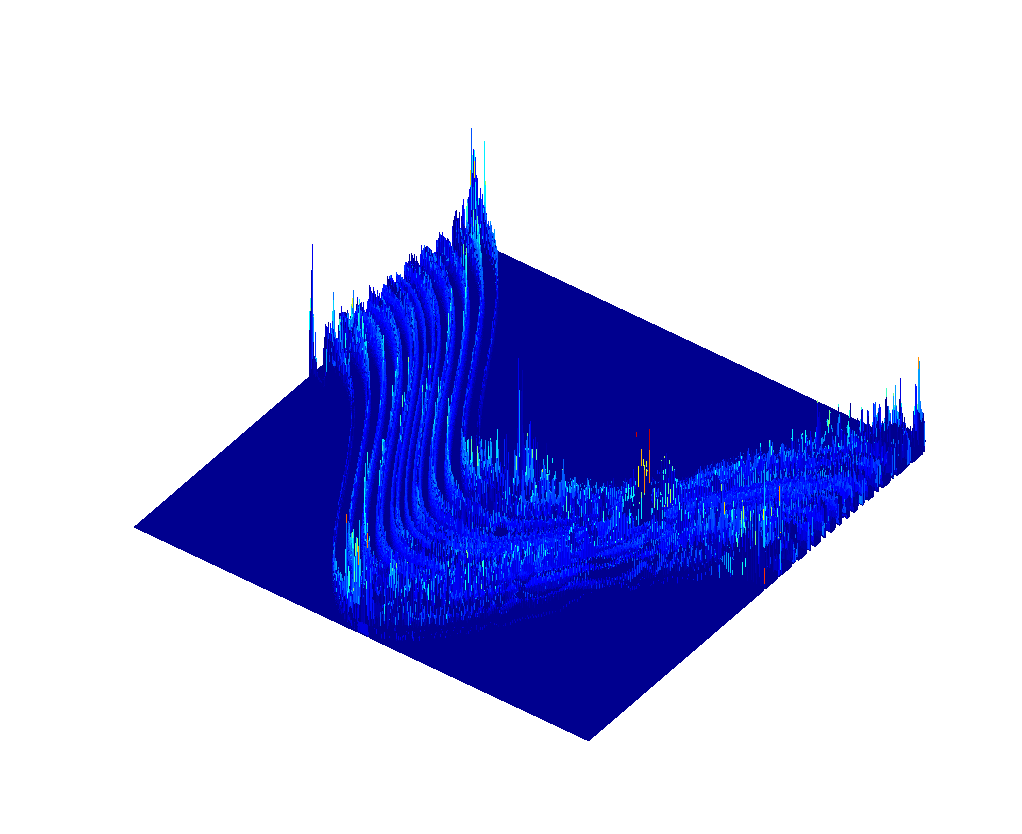
\includegraphics[scale=0.5]{2d_Histogram}
    \label{2d_Histogram}
    \caption{A histogram of $ \nu $ taken from $ 10^6 $ iterations of $ T $ starting at $ \theta_0 = 0.5 $ and $ \nu_0 = 0.5 $ }
\end{figure}

\subsection{}

See code in \emph{Question\_9.m} available at \url{https://github.com/adamjoshuagray/Honours_Ergodic_Theory/tree/master/Assignment_2/Project_1_Code}. (Note we have code from question 9 and 10 together).

We have used the second method outlined above to produce the histogram below in figure 6. We can see that this is probably an exponential distribution (as expected) with parameter = $ 1 / 1140 $.
\begin{figure}[H]
    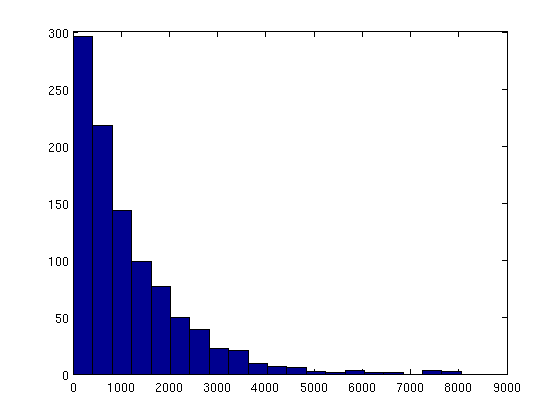
\includegraphics[scale=0.7]{Return_Histogram}
    \label{Histogram}
    \caption{A histogram of the first return time to the high bounce region. }
\end{figure}
\clearpage
\section{}
\subsection{}
See code in \emph{PageRank.m} available at \url{https://github.com/adamjoshuagray/Honours_Ergodic_Theory/tree/master/Assignment_2/Project_2_Code}

\subsection{}
See code in \emph{Question\_2.m} available at \url{https://github.com/adamjoshuagray/Honours_Ergodic_Theory/tree/master/Assignment_2/Project_2_Code}. 

The resultant vector is
\begin{align*}    q =
(  0.011878,
   0.016927,
   0.021698,
   0.021698,
   0.017105,
   0.025485,
   0.013031,
   0.017105, \\
   0.024870,
   0.027504,
   0.039333,
   0.013031,
   0.013898,
   0.025485,
   0.025485,
   0.021174, \\
   0.013031,
   0.013031,
   0.013031,
   0.015050,
   0.103970,
   0.011878,
   0.097454,
   0.111770,
   0.285079
)
\end{align*}
\subsection{}
See code in \emph{Question\_3.m} available at \url{https://github.com/adamjoshuagray/Honours_Ergodic_Theory/tree/master/Assignment_2/Project_2_Code}. 

For $ p = 0.2 $ the resultant vector is
\begin{align*}
    q = (
   0.018891,
   0.020780,
   0.019820,
   0.019820,
   0.020144,
   0.020634,
   0.019139,
   0.020144, \\
   0.020823,
   0.021390,
   0.024838,
   0.019139,
   0.019647,
   0.020634,
   0.020634,
   0.021618, \\
   0.019139,
   0.019139,
   0.019139,
   0.019895,
   0.041789,
   0.018891,
   0.038559,
   0.041962,
   0.453391 
).
\end{align*}
For $ p = 0.5 $ the resultant vector is
\begin{align*}
    q = (
   0.015820,
   0.019775,
   0.019782,
   0.019782,
   0.018879,
   0.021813,
   0.016438,
   0.018879, \\
   0.021982,
   0.023395,
   0.030867,
   0.016438,
   0.017402,
   0.021813,
   0.021813,
   0.021951, \\
   0.016438,
   0.016438,
   0.016438,
   0.018020,
   0.071322,
   0.015820,
   0.065319,
   0.073702,
   0.379674 
).
\end{align*}
\begin{figure}[h]
    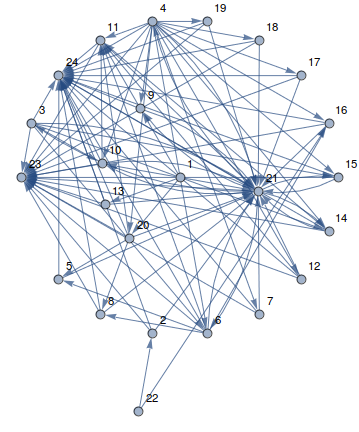
\includegraphics[scale=0.8]{Graph}
    \caption{The layout of the network}
\end{figure}
In figure 7 we see that there are basically 3 important nodes, 21, 23 and 24. When choosing a smaller value for $ p $  we see that across the first 24 nodes the distribution becomes more uniform. If we want to make sure that we keep these nodes as \emph{important} we might choose some intermediate value of $ p $. Say $ p = 0.50 $.
To see a comparison of different weightings given for different values of $ p $ see figure 8. Note that in this figure we have included the $25$-th \emph{Google} node and because this node is connected to every other node by definition it outranks all other nodes. In some sense one should ignore the rank of the \emph{Google} node when assessing the results.

\begin{figure}[h]
    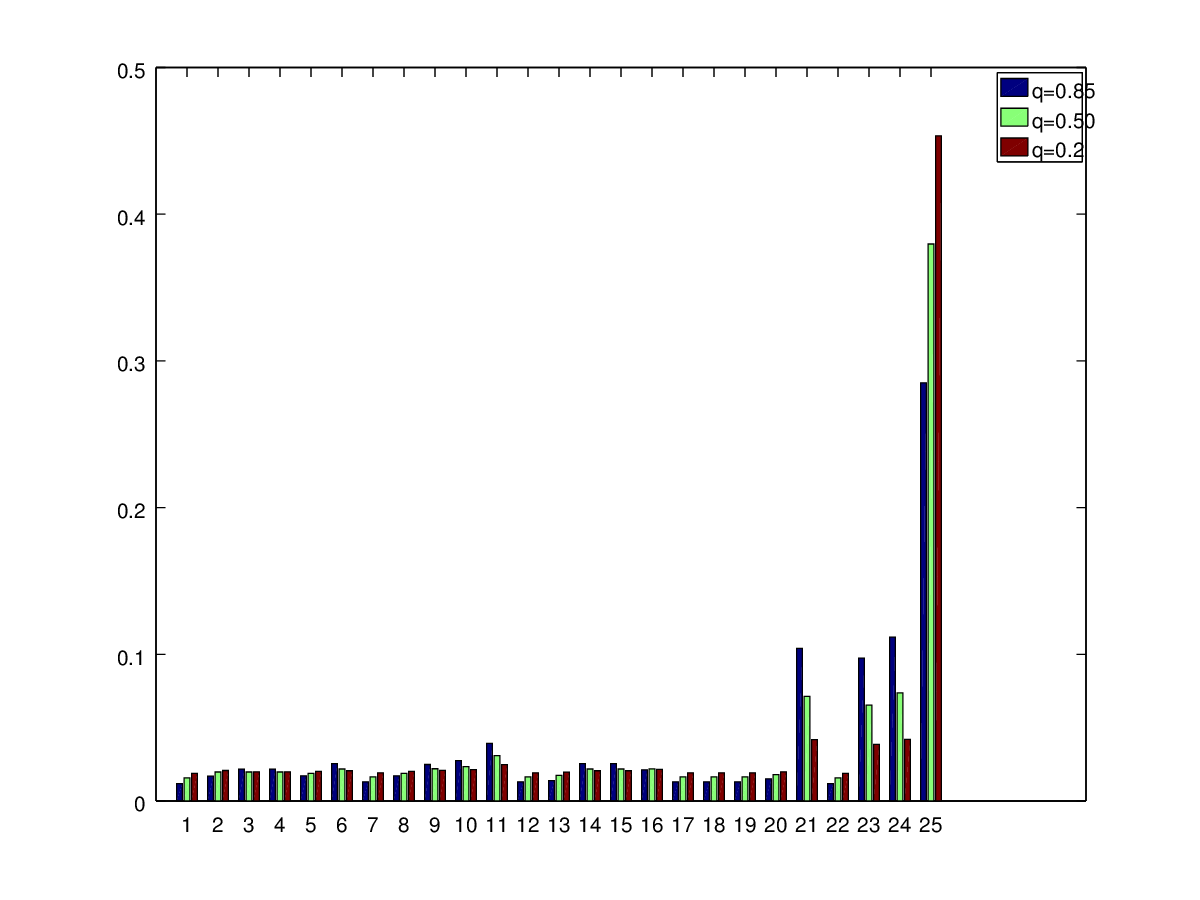
\includegraphics[scale=0.7]{Different_ps}
    \caption{Different weightings for different values of $ p $.}
\end{figure}
\clearpage
\subsection{}
See code in \emph{Question\_4.m} available at \url{https://github.com/adamjoshuagray/Honours_Ergodic_Theory/tree/master/Assignment_2/Project_2_Code}. 

The solution converges exponentially with the error at step n given by
\begin{align*}
    Error(n) = \exp(-0.48640n - 0.25550).
\end{align*}
This is true for about $ n \leq 65 $, after that the error has reached machine precision and cannot improve any further.
See figure 8 for a plot of $ \log(Error(n)) $.

\begin{figure}[h]
    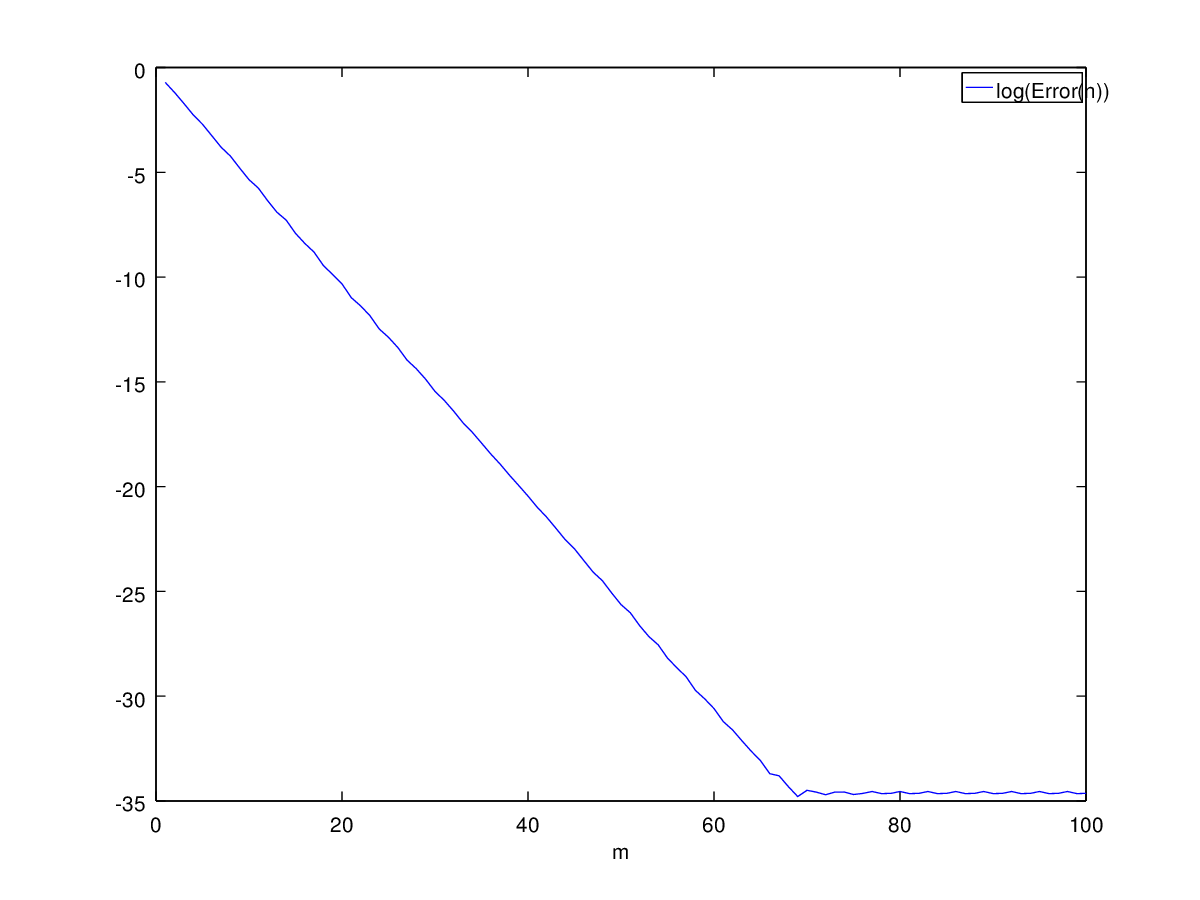
\includegraphics[scale=0.5]{Log_Error_n}
    \caption{Exponential convergence to the stationary vector. Note that at about $n = 65 $ the graph flattens out. This is because the error has reached machine precision.}
\end{figure}

\subsection{}
\subsubsection{}
See code in \emph{PageRank2.m} available at \url{https://github.com/adamjoshuagray/Honours_Ergodic_Theory/tree/master/Assignment_2/Project_2_Code}. 
\subsubsection{}
See code in \emph{Question\_5\_b.m} available at \url{https://github.com/adamjoshuagray/Honours_Ergodic_Theory/tree/master/Assignment_2/Project_2_Code}. 

\begin{align*}
    q = (
   0.023011,
   0.029826,
   0.031190,
   0.031190,
   0.028626,
   0.034984,
   0.024166,
   0.028626, \\
   0.035070,
   0.037710,
   0.051047,
   0.024166,
   0.025737,
   0.034984,
   0.034984,
   0.033940, \\
   0.024166,
   0.024166,
   0.024166,
   0.026891,
   0.124281,
   0.023011,
   0.114333,
   0.129734
)
\end{align*}
\begin{figure}[h]
    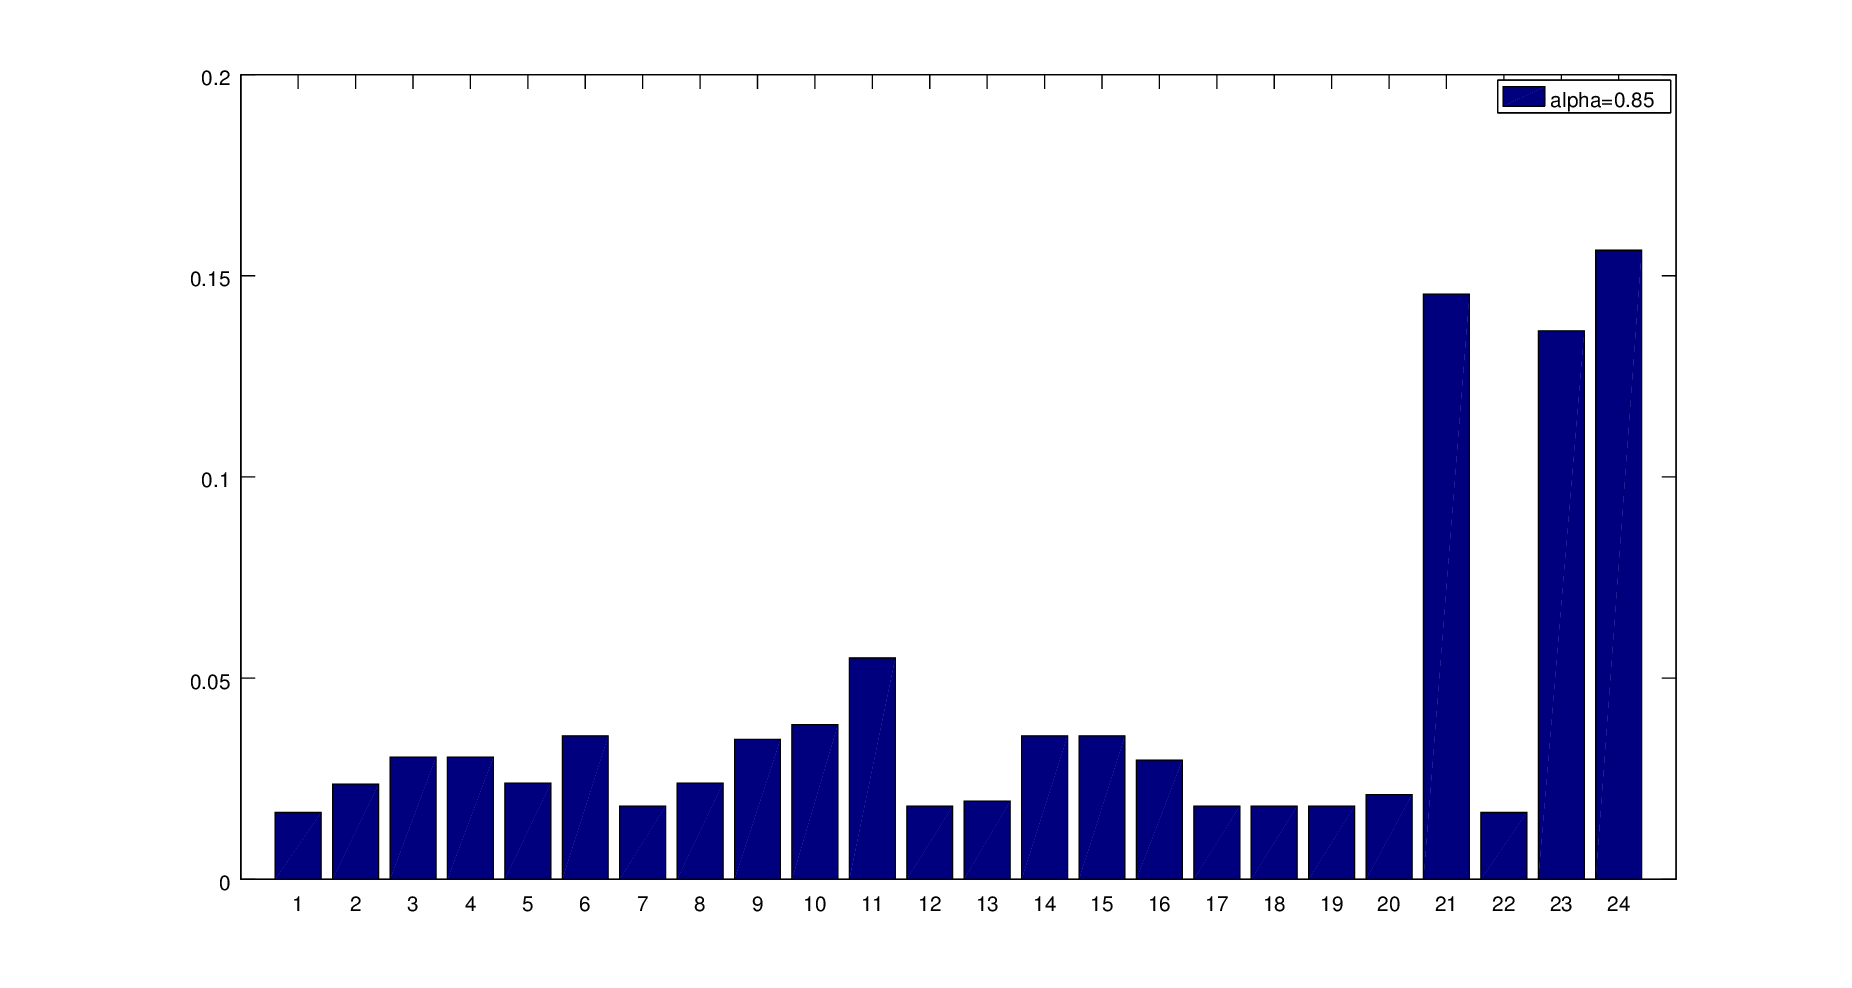
\includegraphics[scale=0.4]{Second_Rank}
    \caption{The page rank weightings for this network using the second page rank algorithm.}
\end{figure}


We can see from figure 10 and by comparing to figure 8, that the this second page rank method results in a more \emph{uniform} distribution or page ranks (we include consideration of the \emph{Google} node in this remark). This is because there is a \emph{latent} connectivity between all pages introduced by the probability of just going to a random page, regardless of the links. This means that each page is \emph{one hop} away from every other page, instead of two hops (via the \emph{Google} node) in the case of the first method. 

If we discard the \emph{Google} node and re-normalise in the $ p = 0.85 $ in the Page Rank vector from the first setup we can observe a perhaps better comparison between the two methods in figure 11. From this we can see that these two methods are essentially equivalent if we discount the \emph{Google} node.

\begin{figure}[h]
    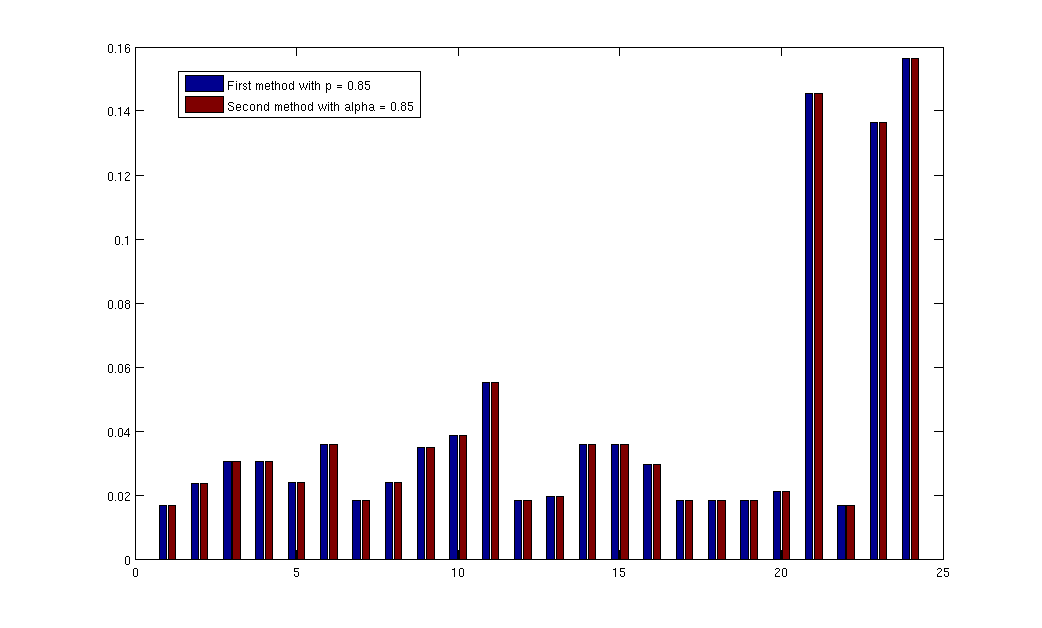
\includegraphics[scale=0.4]{Comparison}
    \caption{A comparison between the first and second methods with $ p = 0.85 $ and $ \alpha = 0.85 $ respectively.}
\end{figure}


\subsubsection{}
See code in \emph{Question\_5\_c.m} available at \url{https://github.com/adamjoshuagray/Honours_Ergodic_Theory/tree/master/Assignment_2/Project_2_Code}. 

The solution converges exponentially with the error at step $ n $ given by
\begin{align*}
    Error(n) = \exp(-1.04629n - 0.25217).
\end{align*}
This is true for about $ n \leq 30 $, after that the error has reached machine precision and cannot improve any further. See figure 12 for a plot of $ \log(Errror(n)) $.

\begin{figure}[h]
    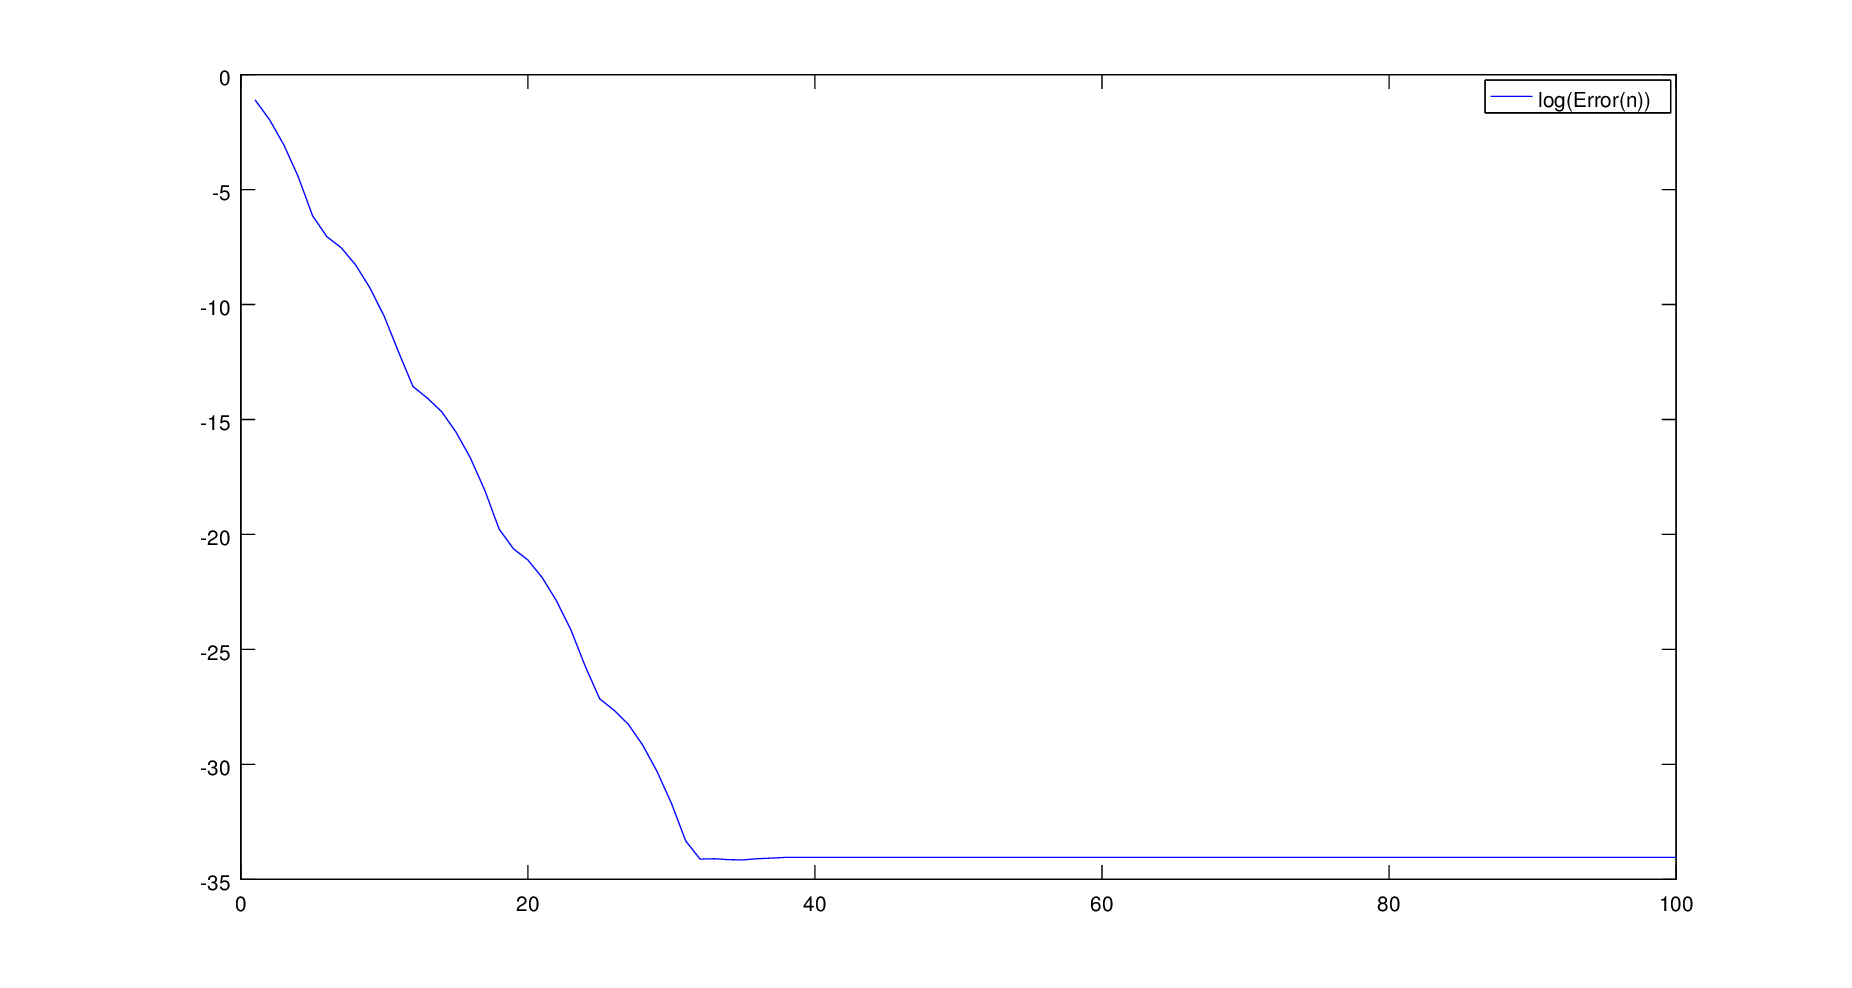
\includegraphics[scale=0.5]{Log_Error_n_2}
    \caption{Exponential convergence to the stationary vector. Note that at about $n = 30 $ the graph flattens out. This is because the error has reached machine precision.}
\end{figure}
It converges faster because the second eigenvalue of $ G $ is $ |\lambda_2| = 0.3511 $ and the second eigenvalue of $ Q $ is $ |\lambda_2|=0.4538 $ and so the power method will converge for $ G $ faster than $ Q $. It also converges faster because the uniform distribution is in a \emph{1 norm} sense, \emph{closer} to $ q $ than in the first case (because the first case has a \emph{Google} node. 
\end{document}
